\documentclass{article}
\usepackage[utf8]{inputenc}
\usepackage{graphicx}
\graphicspath{ {./} }

\title{Assignment 1: Fast Trajectory Replanning}
\author{Jerry Zhu (jlz46)}
\date{Due October 14th}



\begin{document}

\begin{titlepage}
\maketitle
\end{titlepage}

\section{Understanding A*}
a) Explain in your report why the first move of the agent for the example search problem from Figure 8 is to the east rather than the north given that the agent does not know initially which cells are blocked.\\\\
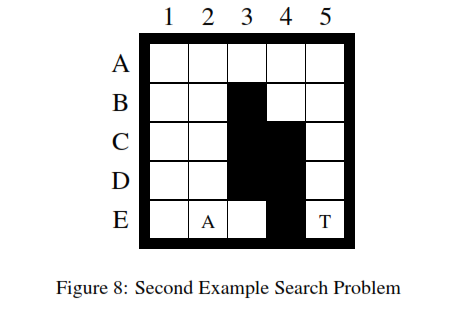
\includegraphics{Figure8.PNG}
Since the agent does not have knowledge of the blocked cells and it only checks for neighbors in the main cardinal directions (North, South, East, West). The agent does not see that there are any walls. With that being the case, the cell to the North has a Manhattan distance of 5 from the goal and the cell to the East has a Manhattan distance of 3. This results in the East cell having the smaller f-value and being the agent's next location (East cell has a f-value of 3 + 1 = 4 whereas North cell has a f-value of 5 + 1 = 6.)\\\\
b) Give a convincing argument that the agent in finite grid-worlds indeed either reaches the target or discovers that this is impossible in finite time. Prove that the number of moves of the agent until it reaches the target or discovers that this is impossible is bounded from above by the number of unblocked cells squared\\\\
First off, the agent will always be able to find out if it is impossible to go from the start to the goal as it calculates the short path, using A*, each time the agent finds a new obstacle. This means that even if the agent has not gone through the entire world if the A* search returns no path then there is no path to be found no matter how far the agent travels. Now when dealing with finding the path to the end the agent will continue to travel towards the goal along the path that was returned by A* until an obstacle is reached and A* is called again to calculate the new path for the agent to take. This means as long as A* returns a path the agent will eventually reach the goal. Now the reason why the the number of moves made my the agent is bounded by the number of unblocked cells squared is because that number is the would be the worst case if the the agent were to look through every single path from every single point.\\\\
\section{Effects of Ties}
a) Repeated Forward A* needs to break ties to decide which cell to expand next if several cells have the same smallest f-value. It can either break ties in favor of cells with smaller g-values or in favor of cells with larger g-values. Implement and compare both versions of Repeated Forward A* with respect to their runtime or, equivalently, number of expanded cells. Explain your observations in detail, that is, explain what you observed and give a reason for the observation.
\\\\When comparing the runtimes of Repeated Forward A* with larger g-values vs smaller g-values, I found tiebreaking in favor of larger g-values produced a much lower runtime. I believe the reason for this is because g-values is a definite value where as the h value is a estimation, being a heuristic. Therefore, choosing a large g-value would give you a smaller h-value which means less estimated distance from the goal.Below are a couple examples of the difference in runtime when looking at gridworlds with valid paths from start to the goal:
\begin{center}
\begin{tabular}{ |c|c|c|c| } 
\hline
Grid & Larger g-values & Smaller g-values \\
\hline
0 & 0.453125 sec & 136.78125 sec \\
7 & 0.359375 sec & 122.25 sec\\
\hline
\end{tabular}
\end{center}
This is a table of expanded
\section{Forward vs. Backward}
a) Implement and compare Repeated Forward A* and Repeated Backward A* with respect to their runtime or, equivalently, number of expanded cells. Explain your observations in detail, that is, explain what you observed and give a reason for the observation. Both versions of Repeated A* should break ties among cells with the same f-value in favor of cells with larger g-values and remaining ties in an identical way, for example randomly.\hfill \break \break
After implementing Repeated Forward A* and Repeated Backward A*, I found that Repeated Backward A* would often find a shorter length path than Repeated Forward A*, however this was not always the case as it is not perfect. While Repeated Backward A* can give a shorter path it does end up taking a little longer in runtime and has more operations. I think because it goes through of the cells, since it works from the goal to the agent, it will provide better paths in many situations. Below are some examples of gridworlds with valid path to from the start to the end: 
\begin{center}
\begin{tabular}{ |c|c|c|c| } 
\hline
Grid & Forward Length & Backward Length \\
\hline
0 & 483 & 379\\ 
7 & 397 & 371\\
10 & 407 & 381\\
11 & 337 & 275\\
\hline
\end{tabular}
\end{center}
\section{Heuristics in the Adaptive A*}
a) The project argues that “the Manhattan distances are consistent in gridworlds in which the agent can move only in the four main compass directions.” Prove that this is indeed the case. Furthermore, it is argued that “The h-values h (s) ... are not only admissible but also consistent.” Prove that Adaptive A* leaves initially consistent h-values consistent even if action costs can increase.\hfill \break \break
The Manhattan distances are consistent because the estimated cost of reaching the goal from the current cell is not greater than than the step cost of getting to its neighbor plus the estimated cost of reaching the goal from that neighbor\footnote{This is in reference to definition given in our textbook Artificial Intelligence A Modern Approach}. This definition is carried over when look at the heuristic for Adaptive A* because even though the action costs can increase the estimated cost will also increase with the current cell. This will keep intact the definition of a consistent heuristic stated before.
\section{Heuristics in the Adaptive A*}
a) Implement and compare Repeated Forward A* and Adaptive A* with respect to their runtime. Explain your observations in detail, that is, explain what you observed and give a reason for
the observation. Both search algorithms should break ties among cells with the same f-value in favor of cells with larger g-values and remaining ties in an identical way, for example randomly.\\\\
After implementing Adaptive A* and comparing it to Repeated Forward A* I found out that Adaptive A* will often find shorter paths than Repeated Forward A*. However with this shorter path it once again encourages a longer runtime as there are more operations and storing within the Adaptive A* algorithm, storing the previous run of A*'s g-score to be used as the heuristic as for the next run of A*. Below are some examples of gridworlds with valid path to from the start to the end: 
\begin{center}
\begin{tabular}{ |c|c|c|c| } 
\hline
Grid & Forward Length & Backward Length & Adaptive Length\\
\hline
0 & 483 & 379 & 453\\
7 & 397 & 371 & 413\\
10 & 407 & 381 & 319\\
11 & 337 & 275 & 337\\
\hline
\end{tabular}
\end{center}
\section{Memory Issues}
a)You performed all experiments in gridworlds of size 101 x 101 but some real-time computer games use maps whose number of cells is up to two orders of magnitude larger than that. It is then especially important to limit the amount of information that is stored per cell. For example, the tree-pointers can be implemented with only two bits per cell. Suggest additional ways to reduce the memory consumption of your implementations further.\\\\ 
When dealing with memory consumption my program could have made some improvements. One improvement I can see is using something better than 2D lists to store most of the information that is being used keep track of the obstacles that the agent has run into. \\\\
b) Then, calculate the amount of memory that they need to operate on gridworlds of size 1001 x 1001 and the largest gridworld that they can operate on within a memory limit of 4 MBytes.\\\\
In Python 3.7.3 and using sys.getsizeof(n) the size of an int object is 14 bytes. Furthermore the size of a list of grid coordinates (eg. [(1,2)]) is 40. With these calculations in mind, there are 2 full grid worlds being stored. This means that there are 40080040 Bytes, or roughly 40 Mbytes, being used to store the values that are being actively used when looking for the shortest path. When working with a smaller size of 4MBytes we can find the largest gridworld by dividing 4000000 Bytes by 40 = 100000. Then taking the square root of 100000 gives a value 316.227766. Therefore, the the largest gridworld that can be used is 316 x 316 gridworld.
\end{document}
